\documentclass[11pt, a4paper,twocolumn]{jarticle}
\usepackage[dvipdfmx]{graphicx}
\begin{document}
%=============================================================
\section{Multibibrator and \\ LED indicator ($2^{nd} day$)}
\subsubsection{Purpose}
単純な電気回路を製作しその動作についてオシロスコープを用いて調べる.
具体的にはシュミットトリガーでNOTゲートを用いて発振器,LEDインジケータを作り,発振器の出力を可視化する.
\subsection{Equipment}
\begin{itemize}
    \item 実験1と同様のもの
    \item Bread board
    \item Oscilloscope and two probes
    \item Resistors (1K$\Omega$,10K$\Omega$,100K$\Omega$)
    \item Ceramic capacitor (0.1$\mu$F)
    \item Aluminum electrolytic \\ capacitor (1$\mu$F,10$\mu$F)
    \item Transistor 2SC1815(GR)
    \item LED (OSDR3113A)
\end{itemize}
\subsubsection{Procedure}
今回の実験以降はブレッドボードによって電気回路を実装していく.
図\ref{fig:8}のように発振器の電気回路を制作する.
multibibratorを作ったらオシロスコープを用いて$V_{in}$,$V_{out}$の値を同時に表示させる.
その後波形をUSBに保存する.
今回は抵抗の値($R_f$)を1K$\Omega$,10K$\Omega$,100K$\Omega$,
コンデンサの容量($C_f$)をそれぞれ1$\mu$F,10$\mu$F
と変化させて測定する.
抵抗,コンデンサの容量をそれぞれ変化させた際の周期の違いを計測する.

次に図\ref{fig:9}に示すようなLEDインジケータの電気回路を制作する.
電気回路が動作するかを確認するために$V_{in}$を5V線につなぎLEDが点灯するか確認する.
その後電圧計により$V_{1},V_{2},V_{3}$の値を計測し,エミッタ電流が20mA以下となっていることを確認する.
発振器回路の出力電圧をLEDインジケータの入力電圧に接続し発振器の出力をLEDを用いて可視化する.
その後LEDの点灯の様子を観察する.

\begin{figure}[htbp]
 \begin{center}
  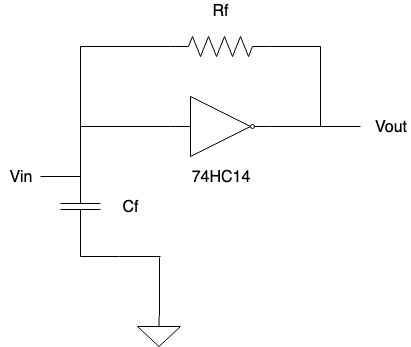
\includegraphics[width=0.8\linewidth]{fig8.png}
 \end{center}
 \caption{multibibrator}
 \label{fig:8}
\end{figure}

\begin{figure}[htbp]
 \begin{center}
  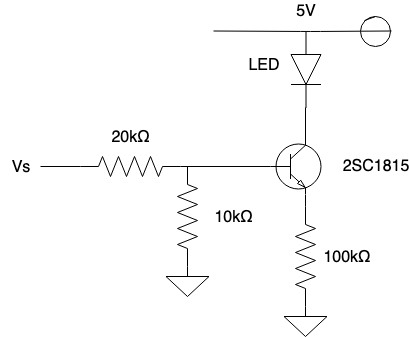
\includegraphics[width=0.8\linewidth]{fig9.png}
 \end{center}
 \caption{LED indicator}
 \label{fig:9}
\end{figure}

\subsubsection{Result}
測定の結果オシロスコープで観察された波形は図\ref{fig:17},\ref{fig:18}のようになった.
またこれ以外の波形に関しては機材の不調によりデータを取れなかったため実験ノートよりそれぞれの場合の周期について表\ref{tab:1}にまとめた.
また全ての$C_f,R_f$において入力電圧は三角波,出力電圧は矩形波となった.

次にこの回路によって生成された出力電圧をLEDインジゲーターの入力電圧としてLEDの光る様子を観察したところ$C_f=1\mu F,R_f=1K\Omega$の時は常に点灯しているように見えた.
$C_f=1\mu F,R_f=10K\Omega$,$C_f=10\mu F,R_f=1K\Omega$の時は高速で点滅しているように見えた.
$C_f=1\mu F,R_f=100K\Omega$,$C_f=10\mu F,R_f=10K\Omega$の時は比較的遅い点滅であった.
$C_f=10\mu F,R_f=100K\Omega$の時はかなり遅く目視で回数が数えられるほどであった.

\begin{figure}[htbp]
 \begin{center}
  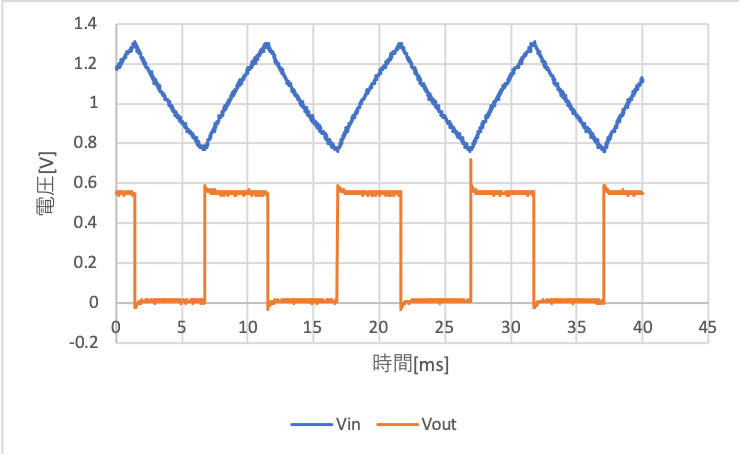
\includegraphics[width=0.8\linewidth]{fig17.png}
 \end{center}
 \caption{$R_f=10k\Omega,C_f=1\mu F$}
 \label{fig:17}
\end{figure}

\newpage

\begin{figure}[htbp]
 \begin{center}
  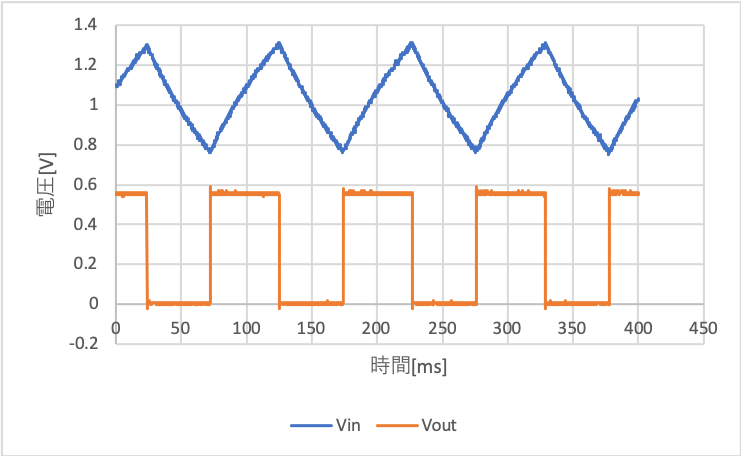
\includegraphics[width=0.8\linewidth]{fig18.png}
 \end{center}
 \caption{$R_f=100k\Omega,C_f=1\mu F$}
 \label{fig:18}
\end{figure}

\begin{table}[htb]
  \begin{center}
    \caption{$C_f,R_f$における$V_{in},V_{out}の周期[ms]$}
    \begin{tabular}{|l|c c c|} \hline
         &$1K\Omega$ & $10K\Omega$ & $100K\Omega$ \\ \hline
      $1\mu F$  & 1 & 10 & 100 \\ \hline
      $10\mu F$ & 10 & 100 & 1000 \\ \hline
    \end{tabular}
    \label{tab:1}
  \end{center}
\end{table}

\subsubsection{Discussion}
まず実験の結果より発振器の生成する矩形波の周波数は
\begin{eqnarray}
    f=C_f\times R_f \nonumber
\end{eqnarray}
によって与えられると考えられる.
次に入力電圧が三角波,出力電圧が矩形波となる理由について考察する.
まず,CMOSのNOTゲートである74HC14には前回の実験結果よりヒステリシス特性があり$V_{in}$が上がっていく際には3V付近に閾値が存在し,$V_{in}$が下がっていく際には2V付近に閾値が存在するという特性があった.
この時の電圧をそれぞれ$V_T^+$,$V_T^-$と名前をつけることとする.

最初に図\ref{fig:8}において初期状態では$C_f$には電荷は溜まってないので$V_{in}$は上昇していくと考えられる.
この時NOTゲートが作動しており$V_{out}$の値は正の値をとる.
その後コンデンサの電圧が上がりNOTゲートにかかる電圧が上がり$V_T^+$に達すると$V_{out}$の値は0となり,それと同時にコンデンサは充電状態から放電状態へと移行し$V_{in}$の値は緩やかに減少していくと予想できる.
以上のことから$V_{in}$は三角波となり,$V_{out}$は矩形波となることが推測できる.

次にLEDインジゲータについて考察する.
まず,LEDが点灯する理由についてはマルチバイブレーターにより生成された矩形波が周期的に正の電圧と0Vの状態繰り返すため,図\ref{fig:9}に示されるトランジスタ(2SC1815)において,マルチバイブレーターから正の電圧が入力される際はベースエミッタ間の電圧が0.6を超えるためトランジスタが作動し結果的にLEDに電流が流れ光るが,一方でマルチバイブレーターから0Vの入力を受け取る際は図\ref{fig:9}のトランジスタが作動せずLEDが点灯しないということが推測される.

次に具体的なケースに分けて考察する.
まず,$C_f=1\mu F,R_f=1K\Omega$の時常にLEDが点灯していたように見えたのはこの時の矩形波の周波数は表\ref{tab:1}より逆数をとってf=1000Hzとなっており1秒間に1000回点滅している計算となるが非常に高速に点滅していたために点灯し続けていたように見えたのだと考えられる.

以下同様に考えると$C_f=1\mu F,R_f=10K\Omega$,
$C_f=10\mu F,R_f=1K\Omega$の時は100Hzとなり点滅が目視可能であると考えられ,結果と矛盾しないと考えられる.

また抵抗とコンデンサの値を変えても一般に$C_f \times R_f$の値が大きくおなるにつれて点滅する周期は徐々に小さくなっていくと考えられる.
%=============================================================
\newpage
\end{document}
